\chapter{iOS Application}

\section{How to install GetALift (GEA) on your iPhone}

\subsection{Xcode}

To work on the GAL project, you have to use Xcode. Xcode downloads directly on the App Store.
\\\\
To open the project on Xcode, launch Xcode and click on \textit{File/Open} and select in the  \textit{getalift-ios} folder the \textit{GALDev.xcworkspace} and click on \textit{Open}

\subsection{GALDev.xcodeprojet}

\begin{figure}[h!]
\begin{center}
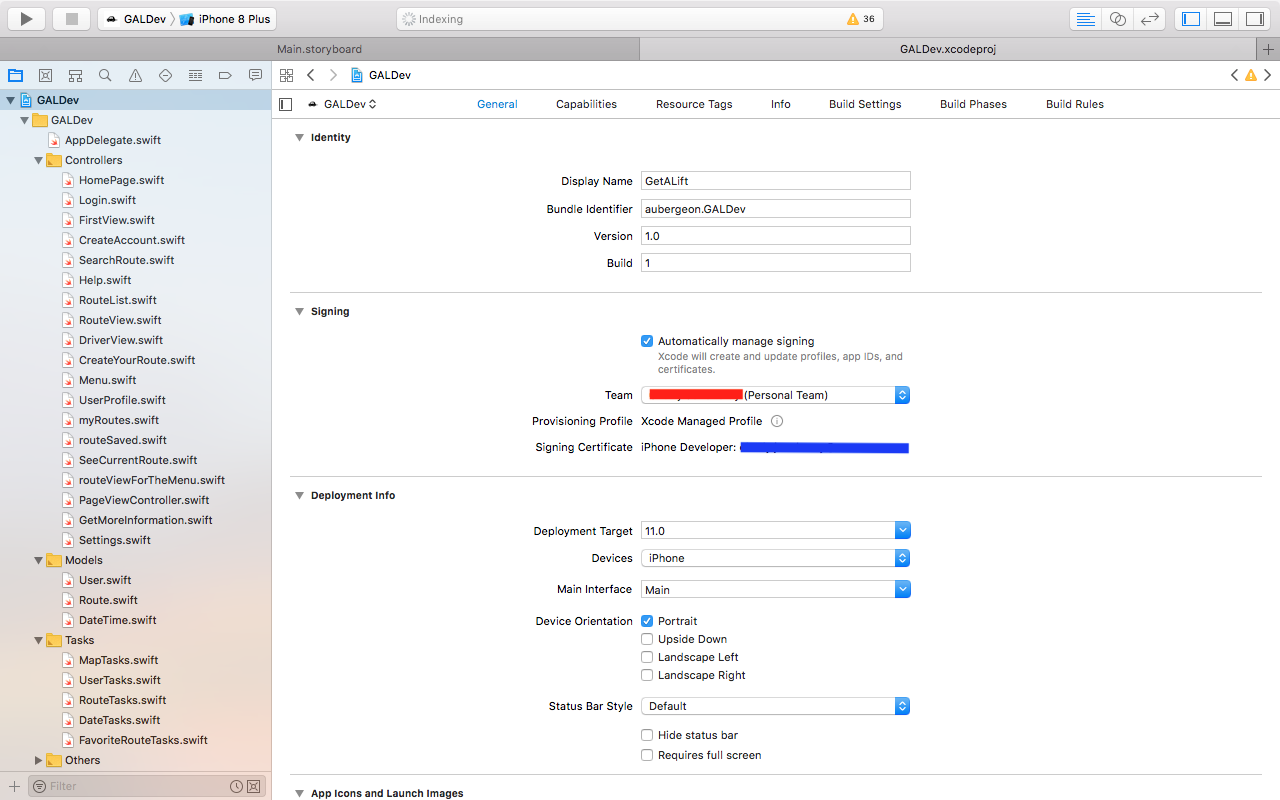
\includegraphics[scale = 0.25]{diagrams/Xcode-General.png} 
\end{center}
\caption{GALDev - General}
\end{figure}
When you open it for the first time you should have errors concerning the \textit{Bundle Identifier}. Take care that it is \textit{yourname.nameoftheproject}.
\\\\
To install the GEA application on your personnal iPhone, you should create a developper account. To create a developper account, go in \textit{Xcode Preferences} and then in \textit{Acount}
\\\\
Click on the "+" and create a new account (cf. figure 5.2). 
\begin{figure}[h!]
\begin{center}
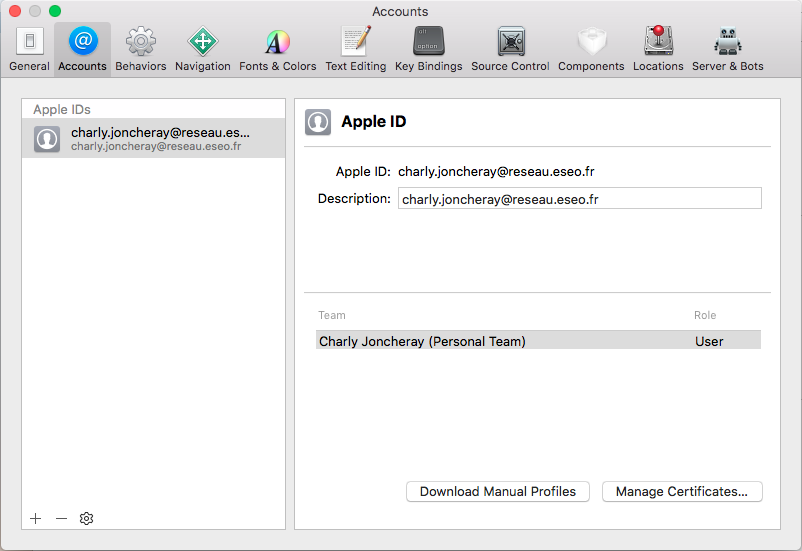
\includegraphics[scale = 0.5]{diagrams/createAnAccount.png} 
\end{center}
\caption{Xcode - Account}
\end{figure}
\\\\
Then, in the \textit{General} page of your project (cf. figure 5.1), select your account as being your \textit{Team} (red box).
\\\\
In the blue box, you should see your email adress.
\\\\
You should have an error concerning the \textit{NotificationBannerSwift}. It because of CocoaPods.

\subsection{CocoaPods}

CocoaPods is a dependency manager for Swift and Objective-C Cocoa projects. It has over 50 thousand libraries. It is used in the GAL application and it is necessary to install it is necessary to install it on your Mac.

\subsubsection{How to install CocoaPods on your Mac}

To install CocoaPods, you have to use the Terminal on your Mac. Open the Terminal.
\\\\
In the folder that contains the project : \textit{/getalift/getalift-ios/} make sure there is the file : \textit{Podfile}
\\\\
If it is not the case, in the Terminal, in the folder containing the xcodeproject file for your project, run the command:
\\\\
\begin{DDbox}{\linewidth}
\begin{verbatim}
pod init
\end{verbatim}
\end{DDbox}
\\\\
This will create a new text file named Podfile (no extension), with the following content:
\\\\
\begin{DDbox}{\linewidth}
\begin{verbatim}
# Uncomment this line to define a global platform for your project
# platform :ios, "7.0"

target 'GALDev' do

end
\end{verbatim}
\end{DDbox}
\\\\
You can delete the first 2 lines of comments. Replace this code by :
\\\\
\begin{DDbox}{\linewidth}
\begin{verbatim}
use_frameworks! #Because we use Swift in the project
target ‘GALDev’ do 
pod 'NotificationBannerSwift'
pod ‘GoogleMaps’
end
\end{verbatim}
\end{DDbox}
\\\\
Then, run the following command line in the Terminal in the folder where the \textit{Podfile} file is located :
\\\\
\begin{DDbox}{\linewidth}
\begin{verbatim}
pod install
\end{verbatim}
\end{DDbox}
\clearpage

\section{GetALift iOS Application}

\begin{figure}[h!]
\begin{center}
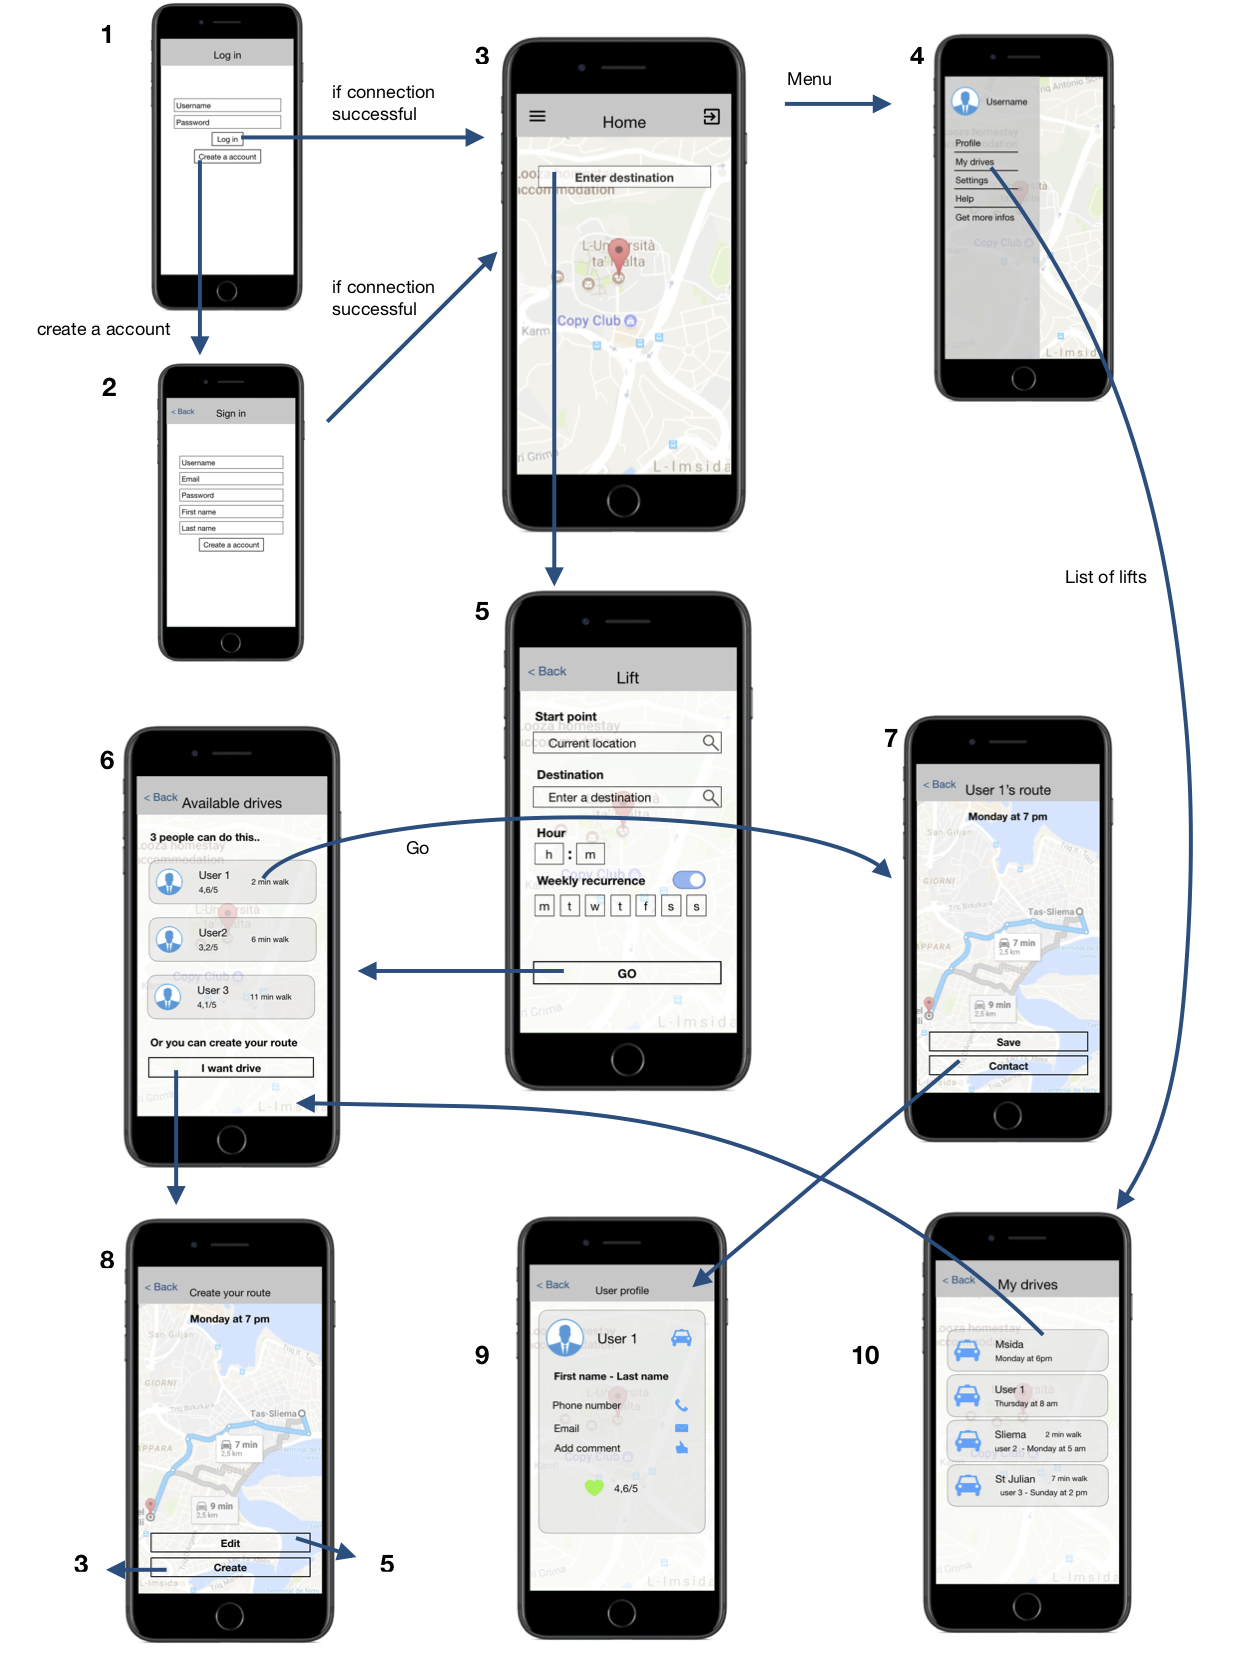
\includegraphics[scale = 0.35]{diagrams/iOSApplication.png} 
\end{center}
\caption{GALDev iOS Application}
\end{figure}

Don't forget to open "GalDev.xcworkspace" in Xcode and not GALDev.xcodeproject otherwise you will have errors.

\subsection{App preview}

\subsubsection{Application homepage}
This is the home page of the app, the one that first appears when the user opens the app. He can access the authentication and account creation page by clicking on the buttons or by making a continuous gesture from left to right on the screen.

\begin{figure}[h!]
\begin{center}
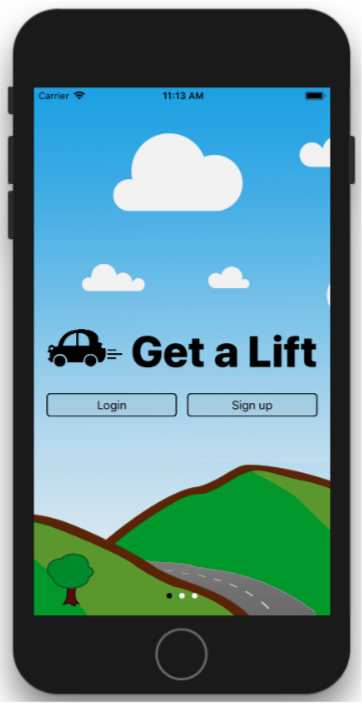
\includegraphics[scale = 0.25]{diagrams/ApplicationHomepage.png} 
\end{center}
\caption{Application homepage}
\end{figure}

\subsubsection{Authentification page}

This page allows the authentication of the user.
\begin{figure}[h!]
\begin{center}
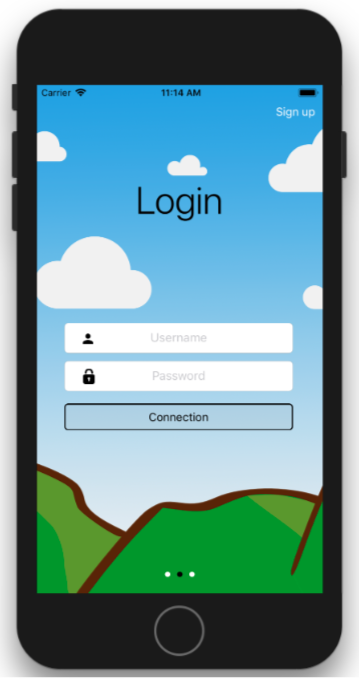
\includegraphics[scale = 0.25]{diagrams/AuthentificationPage.png} 
\end{center}
\caption{Authentification Page}
\end{figure}

\newpage

When the "Connection" button is pressed, the system checks that all the fields are filled in, otherwise it returns an error message in the form of a notification of this type:
\begin{figure}[h!]
\begin{center}

\includegraphics[scale = 0.25]{diagrams/AuthentificationPageFailed.png} 
\end{center}
\end{figure}
\\\\
Then the system sends the collected information to the database which verifies the authentication.

\subsubsection{Account creation page}

This page allows the creation of an user account.
\\\\
\begin{figure}[h!]
\begin{center}
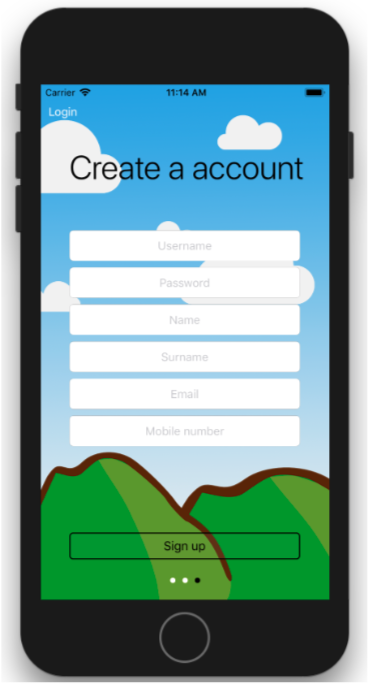
\includegraphics[scale = 0.3]{diagrams/AccountCreationPage.png} 
\end{center}
\caption{Creation Account Page}
\end{figure}
\\\\
When the "Sign up" button is pressed, the system checks that all the fields are filled in, otherwise it returns an error message in the form of a notification.
\\\\
Then the system sends the collected information to the database that creates an account in the database.

\subsubsection{Main page}

Once authenticated, the user arrives on this page, which is the main page of the application. It provides access to the menu and search interface of a route. It also presents a map showing the current position of the user, after authorization of the user.
\\\\
At the top left, there is the button to access the menu and the right is the button to access the search interface of a trip. The button at the bottom right makes it possible to refocus the map on the position of the user.
\\\\
If the user is the driver for routes where the are passengers, alert message will be displayed when he connect. He had to confirm if the passenger was in his car or not. If he click on "Yes", the passenger could see the route in his "MyRides" tab. If he click on "No", the passenger is deleted in the database of the Passenger tab. 

\begin{figure}[h!]
\begin{center}
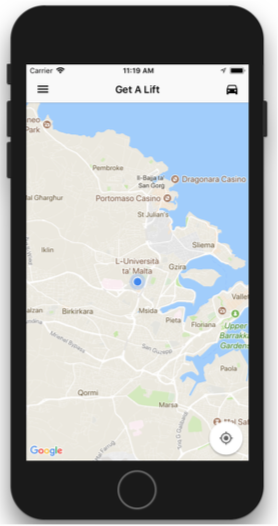
\includegraphics[scale = 0.3]{diagrams/MainPage.png} 
\end{center}
\caption{Main Page}
\end{figure}

\begin{figure}[h!]
\begin{center}
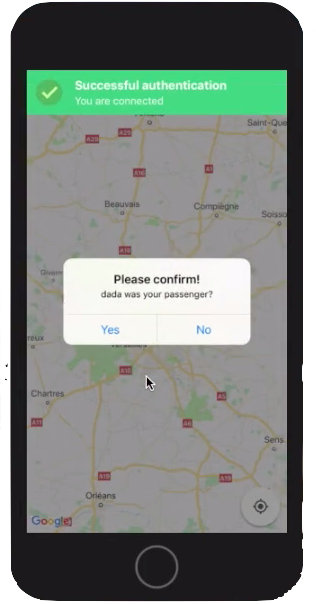
\includegraphics[scale = 0.3]{diagrams/AlertMessage.png} 
\end{center}
\caption{Alert message}
\end{figure}

\subsubsection{Menu}

We can access to different functionality from the menu :
\\\\
We can :
\begin{itemize}
\item go to the main page
\item see information about his profile
\item get more information about the app
\item access a tutorial to discover how the application works
\item access the application settings
\item Sign out.
\item see the section "My routes" which is the list of the routes that the authenticated user has created as a driver
\item see the section "Favorite Routes" which is the list of trips that the user has saved as a passenger.
\item see the section "My Rides" which is the list of the route he made and where his presence was confirm by the driver.
\end{itemize}

\begin{figure}[h!]
\begin{center}
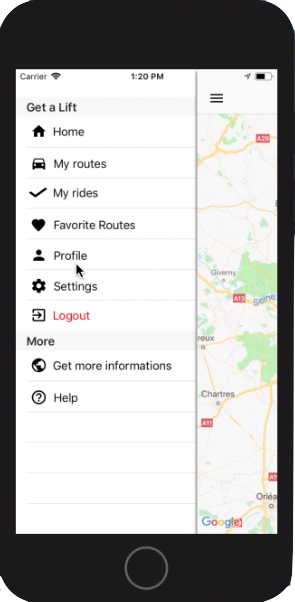
\includegraphics[scale = 0.3]{diagrams/Menu.png} 
\end{center}
\caption{Menu}
\end{figure}

To access the route search interface, click on the button:
\begin{figure}[h!]
\begin{center}

\includegraphics[scale = 0.3]{diagrams/SearchButton.png} 
\end{center}
\end{figure}

\subsubsection{Search interface of a route}

This interface groups together the search and the creation of a trip in order to highlight carpooling. Indeed, if a user wants to create a route as a driver he will in any case access the list of available routes according to his criteria. This will show this user that other people are making the same trip as him and that he is not obliged to create another trip. This makes it possible to promote carpooling and to simplify the use of the application.
\\\\
Here we specify its point of departure and its point of arrival. When you click on the text entry field a drop-down menu is displayed to make suggestions to the user. He can also click on the locate button to display the current position of the user in the text entry field.
\\\\
Once this information is entered, the user can display and fine-tune his journey using a map. By clicking on the "See and edit the route" button.

\newpage

\begin{figure}[h!]
\begin{center}
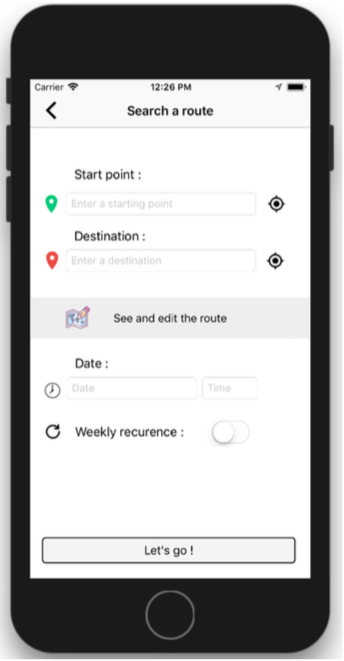
\includegraphics[scale = 0.3]{diagrams/SearchInterfaceRoute.png} 
\end{center}
\caption{Search interface of a route}
\end{figure}

\subsubsection{Preview of the desired route}

On this map you can directly edit the points on the map "by hand". The user can zoom, move the map to draw the path that suits him. Whenever the position of a point is changed, the path between the two points is updated. Once the route has been modified, the user can return to the search page of a trip and the input fields will be immediately modified to display the coordinates of the points he has previously modified on the map.

\begin{figure}[h!]
\begin{center}
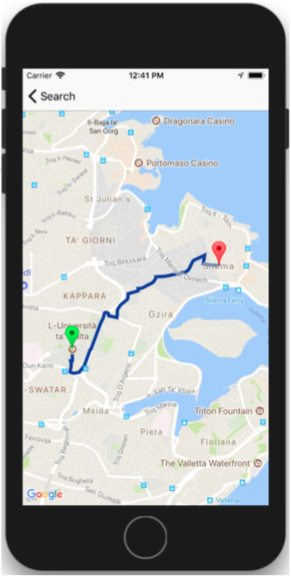
\includegraphics[scale = 0.3]{diagrams/PreviewRoute.png} 
\end{center}
\caption{Preview of the desired route}
\end{figure}

The user can now enter the date and time of his trip in the search interface of a route. He can also notify if his trip will be done every week or not. The purpose of this application is to connect the users of the daily road.
\\\\
Once all fields are completed, he can click on the "Let's go" button to display the corresponding results.
\\\\

\subsubsection{List of available routes}

\begin{figure}[h!]
\begin{center}
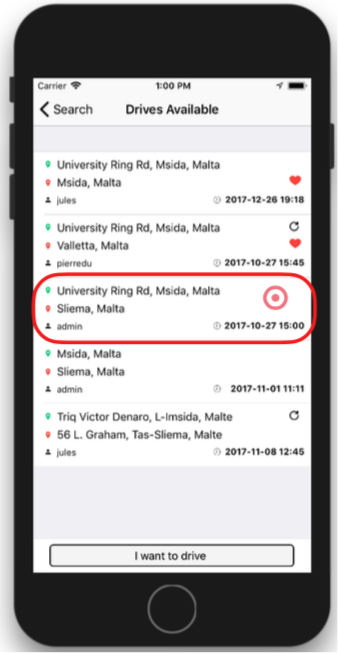
\includegraphics[scale = 0.3]{diagrams/ListAvailableRoutes.png} 
\end{center}
\caption{List of available route}
\end{figure}

We can observe several routes available with information about them (date, time, driver, recurrence). The red heart indicates that it is a road registered as a favorite road.
\\\\
The button offers the possibility to create its own route.
\\\\
If we click on the route, the next page is displayed with the route projection on a map and the different route information.
\\\\

\subsubsection{Overview of a route}

\begin{figure}[h!]
\begin{center}
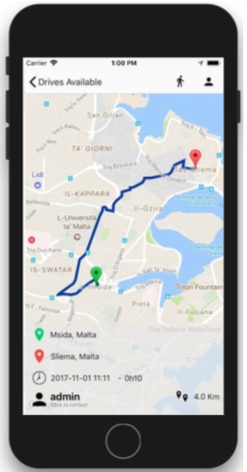
\includegraphics[scale = 0.3]{diagrams/OverviewRoute.png} 
\end{center}
\caption{Overview of a route}
\end{figure}

In this view we find all the information on the trip. We can see the road on a map and if we click on the button representing a man who walks, we will have the way to walk between our starting point and that of the path that will be displayed, and the same for the point of departure. Just press this button again to remove the path to walk.
\\\\
The user can also access the driver's information to contact him or save the trip by clicking on his or her pseudonym or by clicking on the small contact icon at the top right of the screen.
\\\\
If the user will make this route, he can click on the tick button to add this route to his Rides. The rides of a driver are the routes he made. The route will appear in his rides only after that the driver confirm the presence of the user in his car.

\subsubsection{Overview of a driver}

\begin{figure}[h!]
\begin{center}
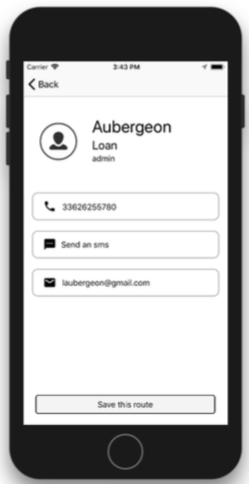
\includegraphics[scale = 0.3]{diagrams/OverviewDriver.png} 
\end{center}
\caption{Overview of a driver}
\end{figure}

The user can call him driver, send him an SMS or an email directly from the application by pressing the dedicated buttons. It can also save this trip to its preferred route list to keep it. He can also see the average of the notes received by the driver and see all the comments let by other users regarding this driver.

\subsubsection{Interface to create a route}

In the case where the user does not find corresponding paths to his trip, he can create a trip by returning to the list of available trips and clicking on the button "I want to drive".
\\\\
We get a summary page of the route that we want to create, if we want to change this it will be enough to go back and change what we want in the search interface / creation. The user presses the "Create your route" button to finalize the creation, a confirmation alert will be displayed on the screen and the user will be redirected to the main page of the application.

\newpage

\begin{figure}[h!]
\begin{center}
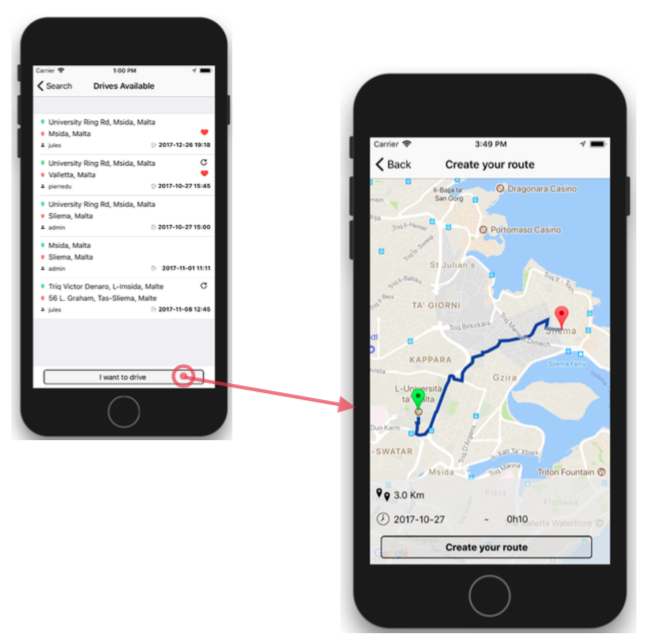
\includegraphics[scale = 0.3]{diagrams/CreateRoute.png} 
\end{center}
\caption{Interface to create a route}
\end{figure}


\subsubsection{List of created routes}

\begin{figure}[h!]
\begin{center}
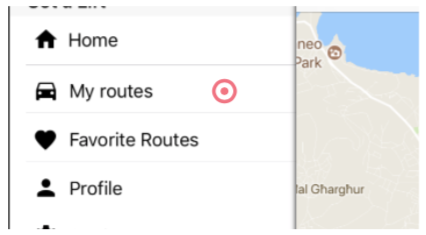
\includegraphics[scale = 0.3]{diagrams/ListCreatedRoute.png} 
\end{center}
\caption{List of created route}
\end{figure}

The user to find this trip in the list of routes he has created, available in the application menu. From this list, the user can see in more detail the routes he has created and delete them.
\\\\
Likewise with the list of his favorite journeys.

\newpage

\subsubsection{List of Rides}

\begin{figure}[h!]
\begin{center}
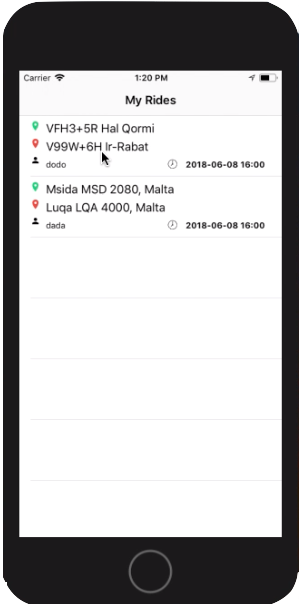
\includegraphics[scale = 0.3]{diagrams/MyRides.png} 
\end{center}
\caption{List of rides}
\end{figure}

The list of rides is the list of the routes that the user made. Since this tab, he can access to the overview of the route he made and to the driver profile.

\subsubsection{Overview of a driver by the tab : "My Rides"}

\begin{figure}[h!]
\begin{center}
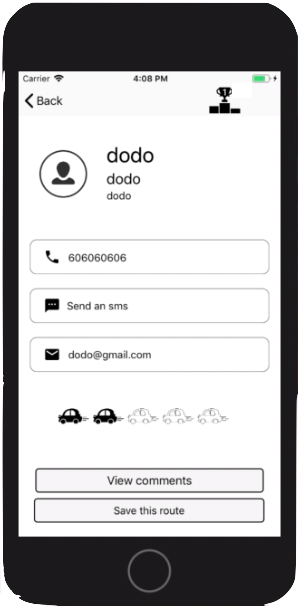
\includegraphics[scale = 0.3]{diagrams/DriverViewRides} 
\end{center}
\caption{Driver View (by passing My Rides tab)}
\end{figure}

The overview of the driver is different when the user display it passing by the My Rides tab. A button appear which allow him to rate and comment the driver.

\newpage

\subsubsection{Rate page}

\begin{figure}[h!]
\begin{center}
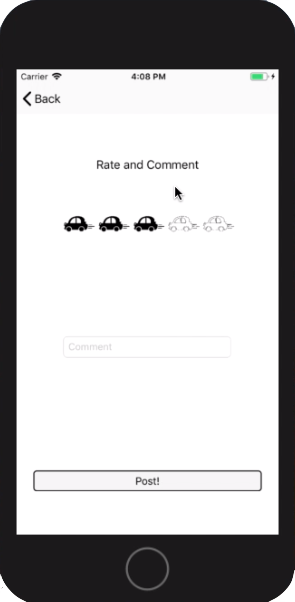
\includegraphics[scale = 0.3]{diagrams/RatePage} 
\end{center}
\caption{Rate page}
\end{figure}

On the rate page, the user can rate and comment the driver. If he already post a comment or a rate, an alert message message inform him that he will modify his rate. He can choose if he want modify his rate or not.

\subsubsection{Comments page}

\begin{figure}[h!]
\begin{center}
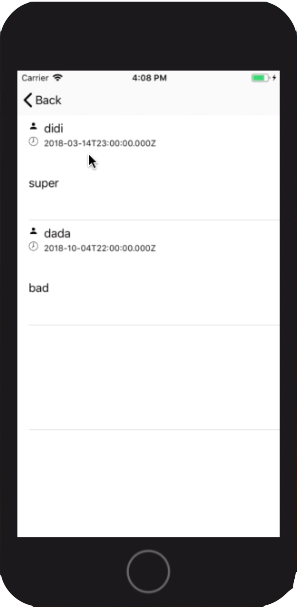
\includegraphics[scale = 0.3]{diagrams/Comments} 
\end{center}
\caption{Comments page}
\end{figure}

On the comment page, the user can display all the comments related to a driver.



\section{GetALift iOS Classes}

\subsection{Model View Controller (MVC)}

MVC is an acronym that stands for Model View Controller. With the VMC, we divide our program into 3 parts:
\begin{itemize}
\item Model: that's what the application does. This is the logic, the brain of the application. He is responsible for the manipulation of the data. In the case of the GetALift application, this part deals with tasks such as saving data, saving, retrieving user data, searching for routes by search parameters, etc.
\item Controller: It retrieves model information and posters in the view.
\item View: that's what the user sees, it's the interface of the application (storyboard)
\end{itemize}

\subsection{Controller}

The code is directly detailed on each corresponding file but this part of the documentation generally describes the classes and their main functions.

In each UIViewController class :

\begin{itemize}
\item the ViewDidLoad function is the function that is called when the page is created.
\item the ViewWillAppear is the function that is called even time that the page appears after it creation
\end{itemize}

\subsubsection{HomePage}

The home page when the user open the application.

\subsubsection{Login}

The first page that opens when the user launch the application.
\\\\
\textbf{Function(s) :}

\begin{itemize}
\item Authentification : This function creates a new user object in the case where the fields "username" and "password" have been correctly completed and the authentication on the backend has 	worked.
\end{itemize}

\subsubsection{FirstView}

The first view of the app when the user is authenticated.
\\\\
\textbf{Function(s) :}

\begin{itemize}
\item createUIAlertController : Create an object of type alert.	

\item showAlert : Display the alert and the 2 actions « Yes » and « No »

\item confirmPassenger : Execute the changeInTheCarColumn request which change the value of the « inTheCar » 		column in the dataBase to confirm the presence of the passenger in the car

\item notConfirmPassenger : Execute the deletePassenger request which delete the user from the database in the case 		where the driver don’t confirm the presence of the passenger in his car.
\end{itemize}

\subsubsection{CreateAccount}

View for that the user create an account on the dataBase.
\\\\
\textbf{Function(s) :}

\begin{itemize}
\item createAccount : This function creates a new user object and a new user in the database in the case where the different fields have been correctly completed and the creation of a new user on the database has worked.
\end{itemize}

\subsubsection{SearchRoute}

The view to research or create a route.

\subsubsection{Help}

Help page.

\subsubsection{RouteList}

The page which display the list of route after a research.

\subsubsection{RouteView}

Class to display the information of an existing route.
\\\\
\textbf{Function(s) :}

\begin{itemize}
\item addToRide : This function execute first the ddRide request. If the POST request works (if « success == true »), a route is associated to a new ride on the database. A passenger is created for the corresponding ride in the database. In the case, where « success == false » which means that an already created ride exist for the current route, there is only a new passenger for the corresponding ride who is created on the database by executing the « addPassengerExistingRide » request.
\end{itemize}

\subsubsection{DriverView}

Class to display information of the driver of the selected route.
\\\\
\textbf{Function(s) :}

\begin{itemize}
\item addToFavoriteRoute : This function execute the addFavoriteRoute request to allow the user to save a route in his Favorite Route tab. If the route is already in your favorite route tab, an error message appears. Otherwise, the route is added to your Favorite Route.	

\item message, mail, phone : Several function in this class allow the user to call, send a message or a mail to the driver
\end{itemize}

\subsubsection{CreateYourRoute}

Class which allow creation of the route on the database and allow the display of the route

\subsubsection{Menu}

\subsubsection{UserProfile}

Class to display the information of the user

\subsubsection{myRoutes}

Class to display the different routes the connected user created

\subsubsection{routeSaved}

Class to display the different routes the connected user add to his favorite routes

\subsubsection{SeeCurrentRoute}

Class to show the route being edited on the research interface

\subsubsection{routeViewForTheMenu}

Class allowing to display informations of an existing route

\subsubsection{PageViewController}

\subsubsection{GetMoreInformation}

Get Morte information page

\subsubsection{Settings}

Settings Page

\subsubsection{Rides}

Class to display the different Rides (route that user made and where the driver confirmed his presence.

\subsubsection{Comments}

Class to display the different comments relative to a driver.

\subsubsection{Rating}

Class which allow to the user to rate and comment the driver for a ride he made. If it is the first time, he rate the driver, it use a POST request and if he modify his rate, it use a PUT request.
\\\\
\textbf{Function(s) :}

\begin{itemize}	
\item rateFunction : This function execute first the postRating request. If the POST request works, the rate is creating in the database and a notification banner inform the user that his rate have been created. If the POST request didn’t work, it means that a rate already exist for this route by the user in the database. The function then execute the putRate function which modify the existing rate if the user click on « Yes » on the alert message which appear or not if he click 	on « No »
\end{itemize}

\subsubsection{EditProfile}

Class which allow the user to modify his personal information on the database.
\\\\
\textbf{Function(s) :}

\begin{itemize}
\item editInformations : This function allow the user to modify his information. The user must to enter his actual password if he want change an information of his profile. If he want to change his password, he must to complete the two fields in the same way or an error banner appears. If his information are correctly modified on the database, a notification banner appears.
\end{itemize}

\subsection{Model}

\subsubsection{User}

This class define the object User

\subsubsection{Route}

This class define the object Route

\subsubsection{DateTime}

This class defines the object date

\subsubsection{Passenger}

This class defines the object Passenger

\subsubsection{Comment}

This class defines the object Comment

\subsection{Tasks}

\subsubsection{MapTasks}

Regroup all the requests concerning the map.

\subsubsection{UserTasks}

Regroup all the requests concerning users.
\\\\
\textbf{Function(s) :}

\begin{itemize}
\item user: Perform GET request which create a user object when it is called.
\item editUser: Perform PUT request which allow to modify an existing user on the database regarding his id
\item authentification: Perform POST request which allow to confirm or not the authentication of a user.
\end{itemize}

\subsubsection{RouteTasks}

Regroup all the requests concerning routes.
\\\\
\textbf{Function(s) :}

\begin{itemize}
\item route POST: It is the POST request which is perform when a user search a route. It create one or several object of type Route in an array to display them after.
\item route (date) GET: Perform GET request which throw back a route regarding it date.
\item route (driverId) GET: Perform GET request which throw back a route regarding it driver.
\item deleteRoute: Perform DELETE request which delete a route regarding it id.
\end{itemize}

\subsubsection{DateTasks}

Regroup all the requests concerning the date.
\\\\
\textbf{Function(s) :}

\begin{itemize}
\item date(routeId): Perform GET request which create a date object regarding the route id when it is called.
\end{itemize}

\subsubsection{FavoriteRouteTasks}

Regroup all the requests concerning favorite routes.
\\\\
\textbf{Function(s) :}

\begin{itemize}
\item favoriteRoute: Perform GET request which create object of type Route regarding the user id to display the different route saved by the user.
\item deleteFavoriteRoute: Perform DELETE request to delete a favorite route regarding the route id.
\item addFavoriteRoute: Perform POST request which save a route regarding a user id in the favoriteRoute tab on the database
\end{itemize}

\subsubsection{PassengerTasks}

Regroup all the requests concerning passengers.
\\\\
\textbf{Function(s) :}

\begin{itemize}
\item passengerNames: Perform GET request that returns a table of all passengers in relation to a driver
\item deletePassenger: Perform DELETE request which allows to delete a passenger according to the id
\item changeInTheCarColumn: Perform PUT request that allows to pass inTheCar to the value 1 if the driver confirms the presence of the passenger
\item addpass: Perform POST request that adds a passenger in the Database regarding the ride Id
\item addPassengerExistingRide: Perform POST request that adds a passenger in the database regarding his id and the route id when a ride already exist regarding the route.
\end{itemize}

\subsubsection{RatingTasks}

Regroup all the requests concerning rates.
\\\\
\textbf{Function(s) :}

\begin{itemize}
\item getRating: Perform GET request which allow to recover the average of the rate o a driver.
\item postRating: Perform POST request which allow to create a rate on the database regarding a driver and a route
\item putRate: Perform PUT request which allow to modify on the database an already existing rate 
\end{itemize}

\subsubsection{RideTasks}

Regroup all the requests concerning rides.
\\\\
\textbf{Function(s) :}

\begin{itemize}
\item rides: Perform GET request hat returns a table of all rides in relation to a passenger.
\item addRide: Perform POST function which create a ride regarding a Route if a ride doesn’t already exist for the route
\end{itemize}

\subsubsection{CommentsTasks}

Regroup all the requests concerning the display of the comments
\\\\
\textbf{Function(s) :}

\begin{itemize}
\item commentaries: Perform GET request that returns all the comments regarding a driver id.
\end{itemize}

\subsection{Others}

\subsubsection{SearchTextField}

Class that manages the operation of the different search bars

\subsubsection{CalculationForMapDisplay}

Class that manage the the display of the map on the screen regarding the zoom.

\subsection{Custom Item}

\subsubsection{MyCustomCell}

Class that manage customCell cells in UITableView

\subsubsection{BoutonArrondi}

Class that manage BoutonArrondi button.

\subsubsection{SelectedButton}

Class that manage the selected button

\subsubsection{BoutonArrondi2}

Class that manage BoutonArrondi2 button.

\subsubsection{RidesTableViewCell}

Class that manage RidesTableViewCell cell in the UITableView table on the Rides page.

\subsubsection{CommentaryTableViewCell}

Class that manage CommentaryTableViewCell cell in the UITableView table on the Comment page.














